\documentclass[letter,10pt]{article}
\usepackage[margin=0.75in]{geometry}
\usepackage{amsmath}
\usepackage{amssymb}
\usepackage{graphicx}
\usepackage{wrapfig}
\graphicspath{ {images/} }
\usepackage{changepage}
\usepackage{collectbox}
\usepackage{polynom} 
\usepackage{color}
\usepackage{indentfirst}
\usepackage{setspace}
\usepackage{algorithm}
\usepackage[noend]{algpseudocode}
\usepackage{clrscode3e}
\RequirePackage{graphics}
\makeatletter
\def\BState{\State\hskip-\ALG@thistlm}
\makeatother
\renewcommand{\baselinestretch}{1}
\setlength{\parindent}{15pt}
\setlength{\parskip}{10pt}

\begin{document}
\vspace*{1cm}
\begin{center} 
\huge
Optimizing Lethbridge Transit Bus Routes
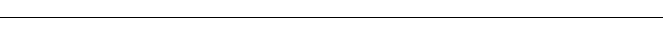
\includegraphics{linebreak}
\vspace*{0.25cm}

\large

\begin{minipage}{0.45\textwidth}
\begin{center}
\vspace*{0.50cm}

Kevin Jia\\
\textcolor{white}{.}\\
Lisgar Collegiate Institute\\
Ottawa, Canada\\
jia.kevin42@gmail.com

\end{center}
\end{minipage}%
\begin{minipage}{0.45\textwidth}
\begin{center}
\vspace*{0.25cm}

Mentor: Dr. Robert Benkoczi\\
\textcolor{white}{.}\\
University of Lethbridge\\
Lethbridge, Canada\\
robert.benkoczi@uleth.ca

\end{center}
\end{minipage}%

\vspace*{1cm}

June 2016

\vspace*{3cm}
\normalsize
\begin{minipage}{0.65\textwidth}
\begin{center}
\textbf{Abstract}\\
\end{center}
This paper proposes methods on how to optimize the bus routes of the City of Lethbridge's transit system, "Lethbrige Transit". Three primary variables are considered in this optimization: distance, turns, and coverage. Given the grid nature of the city, the road system can be projected onto a two dimensional finte, planar, and undirected graph, with intersection as nodes and roads as edges. The method used to compute optimal routes, or paths on the graph, between and through desired bus stops is a modified Dijkstra's Algorithm incorporating Dynamic Programming (DP) and vector calculations. 
\end{minipage}%
\end{center}

\newpage
\section{Introduction}
\onehalfspacing
The problem of finding the optimal path is encountered in everyday life. For example, the average worker needs to plan out the roads he/she will drive on to save the most amount of time possible on daily commutes. This problem is multiplied for transit systems, as buses serve passengers from all across the city that need to travel as fast as possible. Furthermore, given the large nature of a transit system, it is ideal for both citizens and the transit company to have straightforwards, organized routes. This generally encompasses avoiding street changes and turns. Finally, certain local points of interest or stops should be included together in particular routes, as it is desirable to contain local groupings of important locations within routes for ridership convenience and efficiency. This paper proposes an bus route optimization algorithm incorporating these factors.

This paper in particular bases the algorithm on optimizing routes from Lethbridge Transit, the bus system of Lethbridge, Alberta, Canada. It has a population of 94,804 and a size of 2,975.62 square kilometers.[4] The small size results in the curvature of the Earth being negligible, thus allowing Lethbridge to be modelled in a two-dimensional plane. Currently, Lethbridge Transit services 14 routes, 4 stations, and a fleet of 42 buses with the majority of service available 7 days a week. Annual ridership is estimated at 1.1 million.[5]

Using the shapefiles, previous work has been done to create a graph on Lethbridge's road system. This graph details nodes as intersections between two or more roads, and roads as edges. Edge weights are based on the Euclidean distance between the nodes, not the predicted time.

Dijkstra's algorithm is the best known algorithm for the problem in theory and the most robust in practice. The best currently known bounds for the problem, based on a combination of Dijkstra's algorithm and priority queue data structures, is $\Theta ((|E|+|V|)log|V|$. Dijkstra's algorithm solves the Single Source Shortest Path on a graph whose edges have positive length, suiting the requirement that distance between intersections in $\mathbb{R}^2$  must be positive. This algorithm generates a distance table stating the shortest distances to each node from a given node. This is highly effective for finding optimal routes, giving the shortest routes between two desired locations in the city from which the bus will start and stop.

In the proceeding sections, modifications to the basic Dijkstra's algorithm will be proposed to accommodate factors listed above: street changes, turns, and proximity to a list of important locations. All these factors will be balanced with the calculation of a shortest path, by assigning adjustable costs and benefits for meeting certain criteria based on these factors.

The paper is structured as follows: Section 2 discusses background work used in this paper, Section 3 gives the theory used in the modified algorithm, Section 4 describes the implementation of the algorithm, and Section 5 contains concluding remarks and acknowledgements. 

\newpage
\section{Background}
\subsection*{Previous Work}
A previous student has already begun the project by interpreting the raw data provided by the City of Lethbridge. Shapefiles were provided, containing data expressed as vectors: points, lines, and polygons. Using a Python script and a geographic information system, these shapefiles have been converted into a graph. This graph details nodes as intersections between two or more roads, and roads as edges, and contains information on all the roads and intersections in Lethbridge, not just the ones used for bus routes and stops.

The graph is stored a text file, and is stored in the form of adjacency lists. Each list contains information on the node: an unique integer node identifier, 2-D x and y coordinates, and a list of other nodes it is directly connected to. There are approximately 20,000 nodes, and the node identifiers range from 1 to approximately 30,000. The lists are already sorted in ascending order based on the node identifiers. 

To read the graph into whichever program runs the proposed algorithm, a suitable algorithm must be selected. An adjacency matrix is too large as it requires a space complexity of $\Theta (|V|^2)$, and is slow. Thus, leaving it in the form of adjacency lists is suitable. Due to the nature of Dijkstra's algorithm, needing to be able to randomly access memory, an array with the node identifier also being the index is ideal, requiring $\Theta (1)$ time to access a neighbouring node, where as an array/vector without this property would require $\Theta (log\,\, n)$ time by binary search to access a neighbouring node. This thus trades a small increase in memory for a large increase in speed.

\subsection*{Dijkstra's Algorithm}
The problem of finding the shortest path from a specified node s to mother t can be stated as follows:
A simple weighted graph G of $n$ nodes is described by a $n$ by $n$ matrix $D=[d_{ij}]$, where $d_{ij}$ = non-negative weight of the edge from node $i$ to node $j$:
\[ d_{ij} =  \left\{
\begin{array}{ll}
      > 0 & if \, \, i \neq j \\
      = 0 & if \, \, i = j \\
      = \infty \,large \, \, number)& if \, \, \nexists \, \, edge \,\,from \,\, i \, \, to \,\, j \\
\end{array} 
\right. \]

Dijkstra's algorithm labels the nodes of the given graph. The algorithm begins by assigning a permanent distance 0 to the starting node s, and temporary distance of infinity to the remaining $n-1$ nodes. For the first iteration, the current node will be the starting point, and the permanent distance to it will be zero. For subsequent iterations, the current node $i$ will be the closest unvisited node to the starting point. 

\begin{adjustwidth}{1cm}{}

a. Every node $j$ that is directly connected to node $i$ has its temporary distance set to min[current distance of $j$, (distance $i + d_{ij}$)], where $d_{ij}$ is the direct distance between nodes i and j. 

\noindent
b. The smallest, non-infinite value among all the temporary distances is found, and this becomes the permanent distance of the corresponding node. This node becomes the current node $i$. In case of more than one equivalent shortest path, select any one of the candidates to set as the current node.
\end{adjustwidth}

Steps a and b are repeated alternately until there are no more nodes that can be assigned to current node $i$. The permanent distance to any node $j$ is the shortest distance from the source node. The nodes that have unassigned distances have no possible path to the source node.[2]

Proving Dijkstra's algorithm's correctness:

\begin{adjustwidth}{1cm}{}
\textbf{Lemna}: For each $j \in V$, $dist[j] = \delta(j)$, where $j$ is a node, $V$ is the nodes calculated, $dist[j]$ is the calculated distance to $j$, and $\delta(j)$ is the minimum distance to $j$.

\noindent
\textbf{Proof by Induction}: \textit{Base case} ($|V| = 1$): Since $V$ is strictly increasing, the only time $|V| = 1$ is when
$V = \{ source \}$ and $dist[source] = 0 = \delta(source)$, which is correct.

\textit{Inductive hypothesis}: Let $u$ be the last node added to $V$. Let $R' = R \cup \{u\}$. Our I.H. is: for each $x \in R,dist[x] = \delta (x)$.

\textit{Using the I.H.}: By the inductive hypothesis, for every node in $R'$ that isn’t $u$, we have the correct distance label. We need only show that $dist[u] = \delta(u)$, to complete the proof.\\
\indent Suppose for a contradiction that the shortest path from $s$-to-$u$ is $Q$ and has length 
$$\ell (Q) < dist[u].$$
$Q$ starts in $R'$ and at some node leaves $R'$. Let $xy$ be the first edge along $Q$ that leaves $R'$ . Let $Q_x$ be the s-to-x subpath of $Q$. Obviously:
$$\ell (Q_x) +  \ell (xy) \leq \ell(Q).$$
Since $dist[x]$ is the length of the shortest s-to-x path by the I.H., $dist[x] \leq \ell(Q)$, giving us
$$dist[x] + \ell(xy) \leq \ell(Q_x).$$
Since y is adjacent to x, $dist[y]$ must have been updated by the algorithm, so
$$dist[y] \leq dist[x] + \ell(xy).$$
Finally, since u was picked by the algorithm, u must have the smallest distance label:
$$dist[u] \leq dist[y].$$
Combining these inequalities gives us the contradiction that $dist[x] < dist[y].$ Therefore, no such
shorter path Q must exist and so $dist[source] = \delta(source)$. $\blacksquare$

\end{adjustwidth}

Optimal time complexities can be achieved through storing the graph in the form of adjacency lists and using a binary heap (which is how a priority queue is implemented). With these two data structures, the algorithm requires $ \Theta ((|E|+|V|)log|V|)$ [1][3]. Given the size of the city road network's graph, this algorithm is efficient enough to use.
\newpage

\section{Theory}
\subsection*{Calculating Edge Weights}
As stated before, Lethbridge's road network can be considered on a 2-dimensional plane, meaning the Earth's curvature can be ignored. In the undirected graph given, nodes are marked by x and y coordinates and edge weights are not given. Since the graph must be weighted in this scenario, edge weights must be computed. Five scenarios are considered: simple grids, non-uniform grids, curved roads, crescent streets, and loops where the same intersection is linked with itself.

\begin{wrapfigure}{r}{0.2\textwidth}
    \centering
    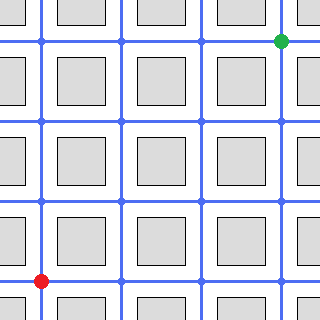
\includegraphics[width=0.2\textwidth]{StreetBlocks1b}
    \footnotesize
    
    Figure 1. Simple grid.
    
    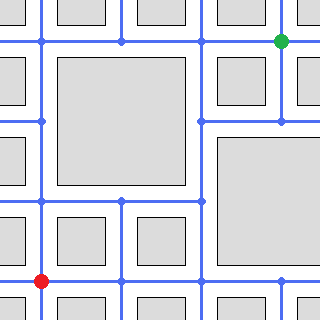
\includegraphics[width=0.2\textwidth]{StreetBlocks2b}
    
    Figure 2. Non-uniform grid.
    
    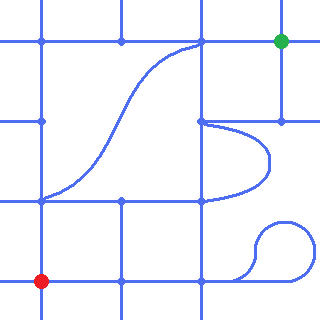
\includegraphics[width=0.2\textwidth]{StreetBlocks3b}
    
    Figure 3. Curved roads, crescents, and loops.
    \vspace{-2cm}
\end{wrapfigure}

Simple grids, like shown in Figure 1, make up the majority of the urban center, and will thus be the most common scenario. Each intersection is clearly connected by a straight line road. Thus, since this is 2-dimensional, edge weights between nodes in this scenario are denoted by their straight-line distance. This distance, D, is given by the formula:
$$D = \sqrt{(x_1-x_2)^2 + (y_1-y_2)^2}$$
where $(x_1,y_1)$ and $(x_2,y_2)$ are the coordinates of the two adjacent nodes.

Non-uniform grids, like shown in Figure 2, are also commonly found in the urban center. This occurs when there are larger blocks than on a simple gird, and will thus omit nodes that would have been there. The remaining intersections and roads remain unaffected, making the distance calculations for the edges the exact same as for simple grids.

Curved roads do not have the same length as the Euclidean distance between the two intersections. However, their curves make them highly irregular and they commonly do not connect adjacent nodes in grids, as shown in Figure 3. Thus, buses will need to change directions. Since the minimum distance between two points is the Euclidean distance in $\mathbb{R}^2$ and curved roads do not have the same length, they must be longer. This increase in distance can be added  approximately to the Euclidean distance through adding a turn cost, which is discussed in the next subsection. Thus, this case is also covered by the distance formula.

Cresent roads, also shown in Figure 3. present an alternate route between two nodes. As stated before, Euclidean distance, which is also the straight line distance, is the shortest route in $\mathbb{R}^2$. Thus, the curved crescent path is longer. Since the algorithm attempts to minimize time, the longer path will be ignored, and the same distance formula is used.

Lastly, loops connecting an intersection to itself, also shown in figure 3, present an option and mathematically makes a multigraph. In every scenario, these loops will be ignored. These loops will clearly have a positive distance. Taking the loop adds a positive distance to the path length and ends on the starting intersection, whereas not taking the loop adds zero distance to the path length and ends on the starting intersection. Since the algorithm attempts to minimize time, the longer path will be ignored, and the loop will be ignored. 

\subsection*{Determining Turns}

Let turns be defined as a change in direction in more than 30 degrees. To check if the next node in a path is a turn or not, the initial movement and the new movement must be known. These can be found using vectors, where if node $c$ is the last node in a path, $n$ is the potential next node to be added into the path, and $p$ is the second last node in the path, the previous direction is $\vec{cp}$ and the next direction is $\vec{nc}$.

Vector calculations can thus be used to find the angle $\theta$ between the two vectors. Note that the dot product of the two vectors has the following two properties:
$$\vec{cp} \cdot \vec{nc} = |\vec{cp}|| \vec{nc} |cos\theta$$
$$\vec{cp} \cdot \vec{nc} = x_{\vec{cp}} \times  x_{\vec{nc}}+ y_{\vec{cp}} \times  y_{\vec{nc}} $$

Since the coordinates of $c$, $n$, and $p$ are given, the $x$ and $y$ coordinates of of $\vec{cp}$ and $\vec{nc}$ are $(x_p - x_c, y_p - y_c)$ and $(x_c - x_n, y_c - y_n)$, respectively. Thus, these two equations can be used to solve $\theta$:
\begin{align*}
\vec{cp} \cdot \vec{nc} &= |\vec{cp}|| \vec{nc} |cos\theta\\
\vec{cp} \cdot \vec{nc} &= x_{\vec{cp}} \times  x_{\vec{nc}}+ y_{\vec{cp}} \times  y_{\vec{nc}}\\
\theta &= cos^{-1} (\frac{\vec{cp} \cdot \vec{nc}}{|\vec{cp}|| \vec{nc} |})\\
&= cos^{-1} (\frac{x_{\vec{cp}} \times  x_{\vec{nc}}+ y_{\vec{cp}} \times  y_{\vec{nc}}}{\sqrt{(x_p - x_c)^2 + (y_p - y_c)^2}\sqrt{(x_c - x_n)^2 + (y_c - y_n)^2}})\\
&= cos^{-1} (\frac{(x_p - x_c) \times  (x_c - x_n)+ (y_p - y_c) \times  (y_c - y_n)}{\sqrt{(x_p - x_c)^2 + (y_p - y_c)^2}\sqrt{(x_c - x_n)^2 + (y_c - y_n)^2}})\\
\end{align*}

On most languages, $cos^{-1}$ gives an answer $0 \leq \theta \leq \pi$, so no turn occurs iff $\theta \leq \frac{\pi}{6}$.

\subsection*{DP on Number of Locations Visited by Paths}
The sub-problem is: given a list of locations and a path, how many of those locations are within $x$ meters of any of the path nodes? Solving this sub-problem allows for the modified Dijkstra's algorithm to optimize the locations visited, where a path "visits" a location if the Euclidean distance between the location and any of the path nodes is less than or equal to $x$, by giving a benefit to visiting a new location.

When solving for a single path, a viable algorithm is to scan through each of the path nodes and locations, and mark each location that has been visited. Given the number of nodes in the path is $|P|$ and number of locations is $|L|$, the time complexity for solving this sub-problem would be $\Theta(|P||L|)$. 

However, this sub-problem needs to be solved for each iteration in Dijkstra's algorithm to account for the differences in locations visited. If the average path length is $p$, the time complexity for the entire algorithm has a time complexity of $\Theta ((|E|+|V|)p|L|log|V|)$. This time required quickly becomes too large on large location sets.

DP can be used to create a faster algorithm that will run in a reasonable time. An array can be created storing the number of locations visited for the determined shortest paths to various nodes $u$. If a call is made to find the number of locations visited for a precomputed path (to node $u$), the number of locations visited can be pulled from the array. 

For finding paths to nodes $v$ that have still not been computed, precomputed solutions can still be used to efficiently compute a answer. In Dijkstra's, only paths that have at most one unvisited node are analyzed. Therefore, paths to node $v$ with $n$ nodes will have a subpath to some node $u$ with $n-1$ nodes, that will have its number of locations visited stored. 

Let the set of nodes visited in the path to node $u$ be $p_u$, and the set of locations visited by a set of nodes $s$ be $L(s)$. The path to $v$ can be expressed as $p_v$ and as stated before, if $v$ is not the source node, Dijkstra's algorithm will give us the property $p_v = p_u \cup \{v\}$ where $u$ is a node for which the locations visited and path has already been caluclated. Furthermore, $|L(p_u)|$ will also be known and stored in the array. By the inclusion-exclusion principle:
\begin{align*}
    L(p_v) &= L(p_u \cup \{v\})\\
    |L(p_v)| &= |L(p_u \cup \{v\})|\\
    &= |L(p_u)| + |L(\{v\})| - |L(p_u \cap \{v\})|\\
\end{align*}

$|L(p_u)|$ is already known. To solve for $|L(p_v)|$, $|L(\{v\})| - ||L(p_u \cap \{v\})|$ must be found. This essentially is the number of locations that $\{v\}$ visits that $p_u$ does not. To do so, first initialize a counter to zero. Then, conduct a simple linear search through the locations and checking if $\{v\}$ visits them, where if it does visit location $\ell$, search through $p_u$ to see if any of those nodes have visited $\ell$. If none have visited $\ell$, increment the counter by one, counting each location that visits $\{v\}$ not $p_u$. After searching through each location, the counter should be equal to $|L(\{v\})| - ||L(p_u \cup \{v\})|$. Therefore, if path $p_u \cap \{v\}$ is chosen in Dijkstra's to be the path to $v$, save index $v$ in the array to be $|L(p_v)|+counter$.

This method reduces the time spent checking whether certain subpaths have already visited locations, saving time. In best case, where the node $v$ does not visit any locations, the time complexity is $\Theta|L|$ for checking a path. This scenario should be the most common, assuming the list of locations is small, since they should be limited to a small area. This time complexity also extends into average time. Only in worst case, where node $v$ visits $\Theta(|L|)$ locations, does it degenerate into $\Theta(|P||L|)$. Therefore, this DP solution is much faster and is employed in the modified algorithm. 

\newpage
\section{Implementation}
To find optimal routes factoring in not only time, but also turns and desired locations visited, a modified Dijkstra's algorithm can be used which employs the theory discussed earlier. Dijkstra's only accounts for distance, and to incorporate turns and locations visited they must be quantifiable. Thus, first assign desired values, in meters, to a turn cost, which will be added to the distance for every turn, and a visit benefit, which will be deducted for every location visited. 

First, a $past$ array is needed. $past[u]$ stores the previous node in the optimal path to node $u$. Since a subpath of $p_u$ to node $v$ is the optimal path to $v$, this array can be used to reconstruct paths from any node back to the source. This can be used to not only return the optimal bus route in the main program, but also in checking locations visited in optimal subpaths.

Let turn cost be given by the function $turn(u,v)$. This function adds the turn cost if the addition of node $v$ to computed path $p_u$ causes another turn. If the number of turns in a path $p$ is $T(p)$, and we extend the definition of $p_{uv}$ to be the subpath from u to v, the equivalence:
$$T(p_v) = T(p_u) + T(p_{uv})$$
always holds true, since a turn is unique and will be only one of the two subsets $p_u$ and $p_{uv}$, since $p_u \cup p_{uv} = p_v,$ and $ p_u \cap p_{uv} = \emptyset$. Therefore, we can include the turn costs into the distances stored in $dist$. 

Let $visited(u,v)$ returns location visit benefit on path to $u$ and node $v$. Note that though the locations visited on the path to $u$ must be stored, which will be done in $locations[u]$, the concept that holds true for turns (ie $T(p_v) = T(p_u) + T(p_{uv})$) does not for location visits, as discussed in the Section 3. Therefore, when comparing potential paths to see if they are faster, $visited$ must be subtracted from each and cannot be incorporated into $dist$ like turn is. This implementation is shown in the pseudocode below in Algorithm 1.

Furthermore, the visit benefit introduces a new problem. Dijkstra's algorithm does not work for negative edge weights. Though the visit benefit does not result in negative edge weights, it causes a similar problem. Visiting a node and then returning to the previous node can result in a negative "distance", and the $past$ array will appear to show an infinite loop. To avoid this, a condition is added such that when comparaing a potential path to see if the new node added $v$ is already in $p_u$. If it is, infinite loops can easily be avoided by immediately discarding this potential path.

Below is the pseudocode for the implementation of this OptimalBusRoute algorithm: 

\newpage
\begin{algorithm*}
\caption{Modified Dijkstra's Algorithm}\label{euclid}
\begin{algorithmic}[1]
\Procedure{OptimalBusRoute}{graph G, source s}
\For{each node $v \in V_g$} 
\State $dist[v] = \infty$
\State $past[v] = undefined$
\State $locations[v] = undefined$
\EndFor
\State
\State $dist[s] = 0$
\State $locations[s] = visited(s,s$) 
\State priority\_queue $pq$ //stores nodes and distance to it, sorts by distance
\State $pq.push(s, 0)$
\State
\While {$pq$ not empty} 
\State $u = pq.extract\_min$
\For{each neighbour $v$ of $u$}
\State $alt = dist[u] + length(u, v) + turn(u, v)$ 
\State $c = length(u, v)$
\If {($alt-c<dist[v]-visited(v,v)$ and $v \notin p_u$)}
\State $dist[v] = alt$
\State $prev[v] = u$
\State $locations[v] = c$
\State $pq.push(v, alt)$
\EndIf
\EndFor
\EndWhile
\EndProcedure
\end{algorithmic}
\end{algorithm*}

In applying this to optimizing bus routes, the graph and the desired locations should be read in through the main program. The turn cost and the visit benefit should also be determined and initialized, at a reasonable value consistent with the scale of the route and the average distance between adjacent nodes. Finally, the $turn$ and $visited$ functions should be written as discussed in Section 3. This implementation, given $|L|<<V$, runs in $\Theta ((|E|+|V|)|L|log|V|)$ time.

\newpage
\section{Concluding Remarks and Acknowledgements} 
In this paper a modified version of Dijkstra's algorithm is presented. The main idea behind these modifications is to make Dijkstra's suitable for optimizing Lethbridge Transit's bus routes. However, this algorithm can be used not just for other bus systems, but also other transportation methods, such as trains, cars, and cruises. The two factors considered, in addition to time, are turns and locations visited from a list of desired locations. Given $|L|<<V$, the proposed algorithm runs in $\Theta ((|E|+|V|)|L|log|V|)$ time.

I would like to thank many people for their assistance in this paper. Firstly, I would like to thank my mentor, Dr. Robert Benkoczi, immensely for presenting this problem, providing previous work, and guiding me on this project. I am extremely grateful that he has taught me so much and answered my questions, despite his busy schedule. I would also like to thank my coop teacher, Ms. Diana Smith, and coop coordinator, Ms. Lauren Sykes, for organizing this coop term. Lastly, I would like to thank Spencer Whitehead for helping me with my code and its bugs.

\subsection*{References}
\noindent
[1] \textcolor{white}{.}Barbehenn, M. (1998). A Note on the Complexity of Dijkstra’s Algorithm for Graphs with Weighted nodes.\\ \indent \textit{IEEE Transactions on Computers}. 

\noindent
[2] \textcolor{white}{.}E. W. Dijkstra. A Note on Two Problems in Connexion with Graphs. \textit{Numer. Math}.

\noindent
[3] \textcolor{white}{.}Goldberg, Andrew V. \& Tarjann, Robert E (1996). Expected Performance of Dijkstra's Shortest Path Algorithm.\\ \indent \textit{NEC Research Institute Report}

\noindent
[4] \textcolor{white}{.}"Population and Dwelling Count Highlight Tables, 2011 Census." Government of Canada, Statistics Canada.\\ \indent \textit{Statistics Canada}, Web. June 2016.

\noindent
[5] \textcolor{white}{.}"Routes and Schedules." Routes and Schedules. \textit{Lethbridge Transit}, Web. June 2016.

\end{document}
